%
% Angepasste FOM Seminarvorlage
%
\documentclass[12pt,a4paper,listof=totoc,bibliography=totoc]{scrartcl}

\usepackage[english]{babel}			% englische Namen/Umlaute
\usepackage[utf8]{inputenc}	    	% Zeichensatzkodierung
\usepackage{fancyhdr}
\usepackage{graphicx}               % Einbinden von Bildern
\usepackage[hidelinks]{hyperref}	% Klickbare Verweise und \autoref{label}
\usepackage[intoc]{nomencl}
\usepackage{setspace}
\usepackage{parskip}
\usepackage{caption}
\usepackage{float}
\usepackage{listings}
\usepackage{geometry}
 \geometry{a4paper, left=40mm, right=20mm, top=40mm, bottom=20mm}
\renewcommand{\familydefault}{\sfdefault}
\renewcommand{\ttdefault}{pcr}
\renewcommand{\lstlistlistingname}{Listings}
\renewcommand{\lstlistingname}{Listing}

% Bildueberschrift oben und rechtsbuendig
\captionsetup{labelfont=bf, textfont=bf}
\captionsetup{justification=raggedright,singlelinecheck=false}

% Blocksatz
\def\justify{%
  \rightskip=0pt
  \spaceskip=0pt
  \xspaceskip=0pt
  \relax
}

%
%	Hier werden Titel, Bearbeiter und das Datum eingetragen
%
\newcommand\svthema{Digital Activism}
\newcommand\svperson{Christian Frank (\#473088)}
\newcommand\svdatum{\today}
\newcommand\lvname{Wirtschaftsinformatik: Web \& Social Media Analytics}
\newcommand\lvtyp{SS 2021}
\newcommand\lvinst{FOM - Hochschule für Oekonomie \& Management}
\newcommand\lvbetr{Gerrit Eicker}

\hypersetup{ % Thema und Author in die Meta-Daten der PDF
  pdftitle={\svthema}, 
  pdfauthor={Christian Frank},
  pdfsubject={Digital Activism - Analysing Blog Performance},
  pdfkeywords={Activism, Web, Analytics, E-Marketing, KPI}
}

\begin{document}

% Titel
\title{ \huge\textbf{\svthema} }
\author{ {\svperson} \\ \svdatum }
\date{ \normalsize \centering 
\includegraphics[width=0.3\textwidth]{FOM}\\ {\lvname} \\ {\lvbetr} \\ {\lvinst} \\ {\lvtyp} }

% Seitennummer oben
\pagestyle{fancy}
\fancyhf{}
\fancyhf[ch]{\thepage}
\renewcommand\headrulewidth{0pt}

\maketitle
\thispagestyle{empty} % laesst die Seitennummer auf der Titelseite verschwinden
\pagenumbering{Roman}

\begin{abstract}
In this paper we will be evaluating the use of Web Analytics to improve community outreach for the for-Future groups during the 2020/2021 Covid-19 Pandemic.

\end{abstract}

\vfill
\begin{figure}[h]
    \centering
    
\includegraphics[]{CC-BY}
\end{figure}

This work is licensed under the Creative Commons Attribution 4.0 International License. To view a copy of this license, visit http://creativecommons.org/licenses/by/4.0/ or send a letter to Creative Commons, PO Box 1866, Mountain View, CA 94042, USA.

\cleardoublepage

\tableofcontents			% Inhaltsverzeichnis
\cleardoublepage

\listoffigures				% Abbildungsverzeichnis
\cleardoublepage

\lstlistoflistings			% Codeverzeichnis
\cleardoublepage

%
% Abkuerzungsverzeichnis
%
\makenomenclature
\renewcommand{\nomname}{List of Abbreviations}

\nomenclature{\textbf{APA}}{American Psychological Association}
\nomenclature{\textbf{COVID19}}{Coronavirus Disease 2019}
\nomenclature{\textbf{DS-GVO}}{Datenschutz-Grundverordnung}
\nomenclature{\textbf{FFF}}{Fridays for Future}
\nomenclature{\textbf{GDPR}}{General Data Protection Regulation}
\nomenclature{\textbf{KFF}}{Kölle for Future}
\nomenclature{\textbf{KPI}}{Key Performance Indicator}
\nomenclature{\textbf{MAPA}}{Most Affected People and Areas}
\nomenclature{\textbf{P4F}}{Parents for Future}
\nomenclature{\textbf{PII}}{Personally Identifiable Information}
\nomenclature{\textbf{RSS}}{Really Simple Syndication}
\nomenclature{\textbf{SQL}}{Structured Query Language}
\nomenclature{\textbf{URL}}{Uniform Resource Locator}

\printnomenclature[1.5in]          % Abkuerzungsverzeichnis
\cleardoublepage

\pagenumbering{arabic}
\setcounter{page}{5}

%
%	Einfuehrung
%

\pagebreak
\section{Introduction}

\onehalfspacing

\subsection{Digital Activism}

In times of Covid-19 climate activisim has partially moved to the digital realm.

Guardian\footnote{\textit{Morresi, E. (2021)}: Protest in a pandemic. \cite{pandemicProtest}} and Guardian\footnote{\textit{Vinter, R. (2021)}: Climate protesters gather in person and online. \cite{climateProtest}} 

Entirely digital \href{https://fffdigital.carrd.co/}{FFF Digital}

\subsection{Gender-neutral Pronouns}

As we move towards a more inclusive and gender-fluid society, it's time to rethink the usage of gendered pronouns in scientific texts. Two well-known professors from UCLA, Abigail C. Saguy and Juliet A. Williams, argue that it makes a lot of sense to use singular they/them instead: "The universal singular they is inclusive of people who identify as male, female or nonbinary."\footnote{\textit{Saguy, A. (2020)}: Why We Should All Use They/Them Pronouns. \cite{pronouns}} Throughout this paper, I'll attempt to follow their suggestion and invite my readers to do the same in future articles, and support an inclusive approach through gender-neutral language. Thank you!
A handy reference to the terms\footnote{\textit{APA (2021)}: Definitions Related to Sexual Orientation. \cite{apaDefinitions}}



%
%	Begrifflichkeiten
%

\pagebreak
\section{Data Source and Wrangling}

\onehalfspacing

\subsection{Data Source}

\subsubsection{The Group}

Kölle for Future is a regional umbrella organization for several for-Future groups in Cologne, mainly Fridays for Future, Students for Future, Parents for Future, Grannies for Future, Teachers for Future, Psychologists for Future, and Scientists for Future.

The group does not have a formal structure but follows the organizational structure of its main actors. As in most grass-roots organizations, most significant decisions are made in plenary sessions, sometimes with majority voting, sometimes through consensus. The decision process is generally speaking not fast - although I got permission to perform the analysis on our blog from the Parents' plenary session, implementing the results of this analysis will take time. Experiments, such as making changes to a form and observing the results, will need to follow the group's decision-making process.

\subsubsection{The Blog}

As part of our overall social media presence and digital activism strategy, we operate a blog for KFF at the following URL: \url{https://koelle4future.de/}.

With our Facebook page and several messenger channels, the blog is the primary medium of broadcasting regional news and events to all for-Futures in and around Cologne.

It is an integral part of our effort to keep the groups together and engaged during the pandemic when we cannot meet in person. Part of the KFF activism has become digital, with bi-weekly virtual rallies (aka \#DigitalStrike) that we hold on Zoom and advertise through the blog. 

In this paper, I will look at the blog's traffic data and analyze that data. The goal is to understand the performance and reach of a blog post based on its content. With this information, we want to improve our outreach and better serve our community.

\subsubsection{Social Media and Loneliness}

Social distancing ("six feet apart") is the critical element of containing the spread of Sars-CoV-2. Unfortunately, it's also the best method to stop the spread, which is easy for some but very difficult for others.

According to a recent study conducted by the American Psychological Association, social distancing over an extended period can increase loneliness and significantly affect people's health.\footnote{See \textit{Luchetti, M. (2020)}: The trajectory of loneliness in response to COVID-19. \cite{apaLoneliness}}

In their study, the researchers hypothesized that an increase in support from others, perceived or actual, can significantly offset that feeling of loneliness.

One means to support the members of our community is through an increase in interaction on social media. To maximize outreach, we use all kinds of channels in parallel and include a blog. We hope that the more engaging a blog post is, the better are its chances to reach people and be entertaining or otherwise beneficial. The main goals are to keep our community engaged and to combat loneliness.

Another means to reach out to our community is through virtual meetings with video. However, here we will not look into this or in any other channel than our blog.

\subsubsection{Hate Speech}

Besides loneliness, another aspect of moving to the digital realm in the Covid-19 pandemic is an increase in Hate Speech, especially in social media. We aim to offer a safe and welcoming digital space in our blog and our other platforms and restrict the use of hateful words in comments and derogatory terms.

With Covid-10, as with any other illness, comes stigma, and we need to be especially aware not to stigmatize people who have contracted the virus and might be on a long path to recovery.\footnote{See \textit{UNAIDS (2020)}: Addressing stigma and discrimination. \cite{addressingStigma}} During the pandemic, it's imperative to be inclusive to all people, inside and outside of our community.\footnote{See \textit{TIME's UP (2020)}: Equity and Inclusion During Crisis. \cite{equityInclusion}}

\subsubsection{Ableism}

There is also an increase in violence in the written language\footnote{See \textit{Brown, L.X.Z. (2014)}: Violence in Language. \cite{violenceLanguage}}, with an increase in the use of derogatory ableist terms. A good example is the term "Covidio***", which is ableist and should not be used, according to the scientist Jason von Juterczenka.\footnote{See \textit{Juterczenka, J.v. (2021)}: Begriff "Covidio***". \cite{covidioXXX}}

Being mindful in communication, online and offline, requires careful evaluation of the terminology we use in our posts and comments. Sometimes it also requires a certain level of restraint. For our communication, we use a handy reference to ableist terms\footnote{See \textit{Brown, L.X.Z. (2021)}: Ableism/Language. \cite{ableismLanguage}} that we want to avoid.

\subsubsection{Climate Anxiety}

We need to place special consideration on climate anxiety with the for-Future groups. The knowledge and understanding of the coming climate catastrophe can be overwhelming and lead to anxiety attacks and depression. As a group, we aim to spread as much a positive image and outlook on the future as possible. We do not want to overwhelm our community, but at the same timem we need to focus on the necessity of immediate action and convey a sense of urgency.

According to a recent study, the group in Cologne is mainly White, an issue that a lot of for-Future groups in the Global North have, and we are thus prone to a higher level of anxiety.\footnote{See \textit{Dellinger, AJ. (2021)}: The connection between climate anxiety and white fragility. \cite{climateAnxiety}}

\subsection{Web Traffic Analysis}

\subsubsection{Web Traffic KPIs}

Web analytics belongs to the domain of the big search engines, and Google Analytics is the market leader. Web analytics plays a significant role in evaluating a website's performance.

As a marketing category, a blog is considered inbound marketing. It tries to offer interesting content and engage its readers, but it does not reach out by itself. Yvonne Romes identifies a couple of important KPIs for inbound marketing.\footnote{See \textit{Romes, Y. (2020)}: 10 Inbound KPIs, die jetzt auch Personaler kennen sollten. \cite{inboundKPI}}

Unfortunately, not a lot of these KPIs are present in our blog's metrics. I will hence focus on the metrics that the statistics module offers. To analyze the data, I will mainly use visualization and correlation to identify areas where we could improve the blog's outreach.

\subsubsection{Data Collection}

We collect metrics for the Kölle for Future Blog on the web host itself; we are not using an external service, such as Google Analytics or Plausible for this. We host the blog on WordPress in a virtual private instance.

To collect metrics, we use the wp-statistics plugin\footnote{See \textit{VeronaLabs OÜ (2021)}: Documentation. \cite{wpStatistics}} which stores its data in Wordpress' MariaDB database.

I exported the data from the blog as CSV files for analysis.

\subsection{Data Wrangling}

\subsubsection{Original Columns}

We have six files in total. First, let's have a look at each of the files' contents and the original columns.

The wp-admin table covers the admin access to the blog instance.
\begin{lstlisting}[caption=wp-admin, frame=single, basicstyle=\ttfamily]
"date", "IP", "hostname"
\end{lstlisting}

The wp-comments table holds all information pertaining to comments, which will greatly help us in evaluating engagement with the individual posts.
\begin{lstlisting}[caption=wp-comments, frame=single, basicstyle=\ttfamily]
"comment-ID", "comment-post-ID", "comment-author", 
"comment-author-email", "comment-author-url", 
"comment-author-IP", "comment-date", "comment-date-gmt", 
"comment-content", "comment-approved", "comment-parent", 
"comment-type", "user-id", "comment-alter-id", 
"meta:ct-checked", "meta:ct-checked-now", "meta:ct-bad", 
"meta:ct-hash", "meta:akismet-result", 
"meta:akismet-history", "meta:akismet-as-submitted"
\end{lstlisting}

The wp-pages table has all individual wordpress pages and posts and the number of impressions; "id" links to "comment-post-ID" i wp-comments.
\begin{lstlisting}[caption=wp-pages, frame=single, basicstyle=\ttfamily]
"page-id", "uri", "type", "date", "count","id"
\end{lstlisting}

The wp-search table contains information of search engine referrals; "visitor" links to the "id" of wp-visitor.
\begin{lstlisting}[caption=wp-search, frame=single, basicstyle=\ttfamily]
"ID", "last-counter", "engine", "host", "words", "visitor"
\end{lstlisting}

The wp-visits table shows total number of visits per day.
\begin{lstlisting}[caption=wp-visit, frame=single, basicstyle=\ttfamily]
"ID", "last-visit", "last-counter", "visit"
\end{lstlisting}

The wp-visitors table has the information for each unique visitor and links all other tables together.
\begin{lstlisting}[caption=wp-visitor, frame=single, basicstyle=\ttfamily]
"ID", "last-counter", "referred", "agent", 
"platform", "version", "UAString", "IP", 
"location", "user-id", "hits", "honeypot"
\end{lstlisting}

\subsubsection{Removing PII}

There's quite a lot of personally identifiable information in these tables that I will remove before starting the analysis:

\begin{itemize}
 \item wp-admin: The information in this table is only affecting me as the author of the paper, so no change is necessary
 \item wp-comments: I'll remove anything that could potentially identify the person commenting as well as all meta information and an empty column.
 \item wp-pages: The table has no personally identifiable information
 \item wp-search: The table has no personally identifiable information
 \item wp-visit: The table has no personally identifiable information
 \item wp-visitor: I'll remove all information, including IP Address, that could potentially identify the visitor
\end{itemize}

Removing columns from CSV files is an easy task for any spreadsheet program.

\subsubsection{GDPR Compliance}

We can assume that wp-statistics is not GDPR-compliant from the amount of data that we need to remove, even though it claims that it is.\footnote{See \textit{Kohr, J. (2020)}: Matomo vs. WP-Statistics. \cite{matomoBlog}} Furthermore, there is no information visible on the blog that we will process personal data, as required by DS-GVO. The collection of IP addresses is challenging to justify and completely unnecessary. 

To achieve GDPR compliance and continue analysis, I will recommend the following actions for the plugin configuration:

\begin{itemize}
 \item Enable Geo-IP location data
 \item Disable collection of IP addresses
\end{itemize}

\subsubsection{Removing Spam}

Spam is a big issue for WordPress blogs; the blogs are easily identifiable on the web and share common vulnerabilities; we can safely assume that our blog is prone to spam access. The blog's language is German, so I think that access from non-German speaking countries is likely to be fraudulent. It is a broad assumption and might exclude legitimate traffic. Still, for this paper, I will go with the hypothesis and remove traffic from countries other than Germany, Austria, and Switzerland.  

To do this I use the shell and filter approximately 18000 page impressions:

\begin{lstlisting}[caption=Removing Spam, frame=single, basicstyle=\ttfamily]
$ wc -l wp-visitor-2021-04-05.csv
68027 wp-visitor-2021-04-05.csv

$ fgrep -e "DE" wp-visitor-2021-04-05.csv | wc -l
49883

$ fgrep -e "AT" wp-visitor-2021-04-05.csv | wc -l
519

$ fgrep -e "CH" wp-visitor-2021-04-05.csv | wc -l
264

$ fgrep -e "CH" -e "AT" -e "DE" wp-visitor-2021-04-05.csv \
  > wp-visitor-2021-04-05-nospam.csv

$ wc -l wp-visitor-2021-04-05-nospam.csv 
50564 wp-visitor-2021-04-05-nospam.csv
\end{lstlisting}

\subsubsection{Count Data Notebook}

Now that we have removed all PII items and filtered spam, it's time to analyze the data. To do this, I'll again use a data notebook from Count.

Count data notebooks combine SQL data and text quickly, much like Jupyter notebooks combine Python code and text. Count aims to support teams with data-driven decision-making and has recently come out of open beta.\footnote{See \textit{Count.co (2020)}: About Count. \cite{aboutCount}}

To load the tables into the data notebook, I created a BiqQuery database on my Google Cloud instance and connected the Count data notebook with a read-only service account. As a final results, here's the list of tables for the notebook:

\begin{figure}[H]
\centering
\caption {Database Tables}
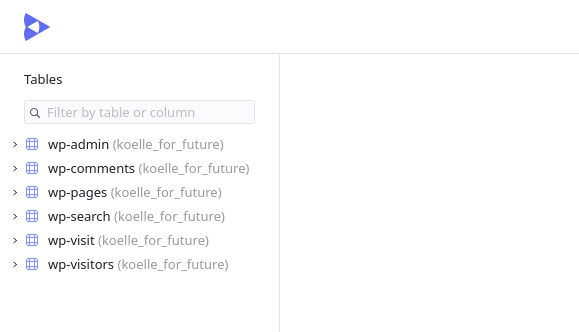
\includegraphics[width=\linewidth]{images/tables.png}
\label{fig:tablesCount}
\end{figure}

Count notebooks make exploration of data accessible. Unfortunately, the internal format is Markdown, and import into LaTeX is not entirely without problems; in the end, it did work for the following two chapters. Count also no longer allows anonymous (read) access to the notebooks; otherwise, I would have shared the link here.


%
%	Theorieteil
%

\pagebreak
\section{Data Exploration}

\onehalfspacing

\subsection{Access}

Now that we have all the data from wp-statistics in our BigQuery tables, we're ready to start the exploration. 

Let's start by looking at the number of visitors this year. We can see a huge spike around the global climate strike on March 19 and a smaller one before Easter:

\begin{figure}[H]
\centering
\caption {Visitors 2021}
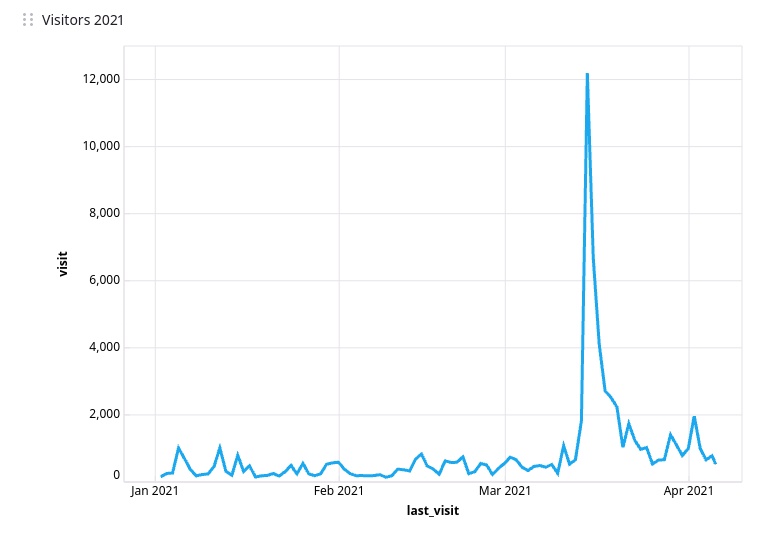
\includegraphics[width=\linewidth]{images/figure01.png}
\label{fig:visitors2021}
\end{figure}

A global climate strike is a significant event in our groups' calendar, and I am pretty happy that we were able to provide our readers with sufficient information about it.

Let's move to the past year. We can see similar significant spikes around the dates for global and local strikes, and local elections:

\begin{figure}[H]
\centering
\caption {Visitors 2020}
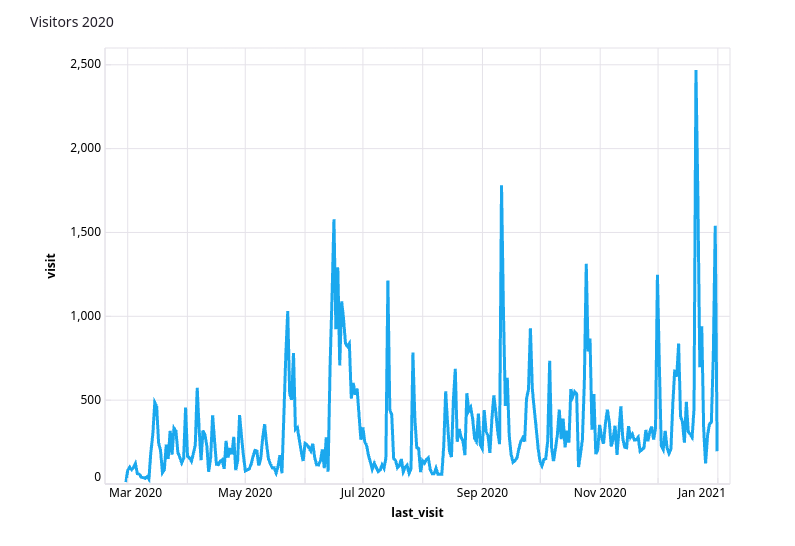
\includegraphics[width=\linewidth]{images/figure02.png}
\label{fig:vistors2020}
\end{figure}

The external calendar data again correlates with the access data; the blog thus seems to fulfill an essential role in keeping our community informed and engaged.

\subsection{Search Engines}

In addition to the people who have bookmarks for the blog, a significant amount of traffic comes from the major search engines:

\begin{figure}[H]
\centering
\caption {Search Engines}
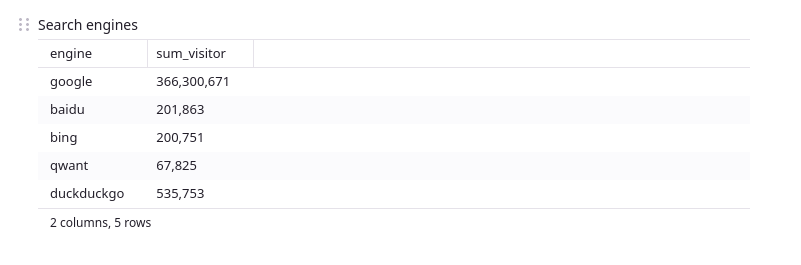
\includegraphics[width=\linewidth]{images/figure03.png}
\label{fig:searchEngines}
\end{figure}

Google is the market leader, but DuckDuckGo is a (distant) runner-up, and we'll see DuckDuckGo again a little bit further down.

Looking at the main key words, we find "Klimastreik" (climate strike) and "Wahl" (local elections) in various forms in our data:

\begin{figure}[H]
\centering
\caption {Search Term Streik}
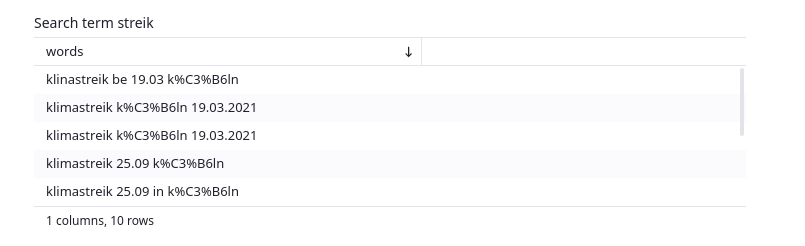
\includegraphics[width=\linewidth]{images/figure04.png}
\label{fig:searchStreik}
\end{figure}

\begin{figure}[H]
\centering
\caption {Search Term Wahl}
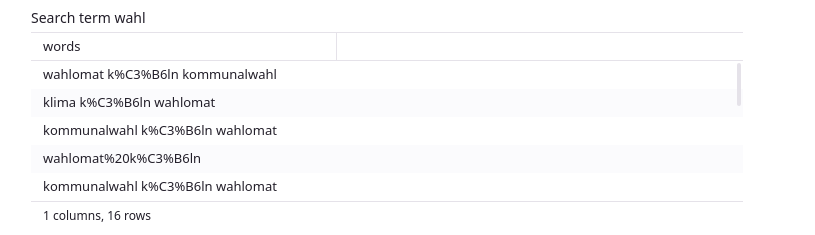
\includegraphics[width=\linewidth]{images/figure05.png}
\label{fig:searchWahl}
\end{figure}

This data supports our findings so far that people inside and outside the community turn to the blog for information for the regular climate strikes and the local elections.

\subsection{Admin Access}

Because we have the data, let's have a look where our admin users come from:

\begin{figure}[H]
\centering
\caption {Admin Access}
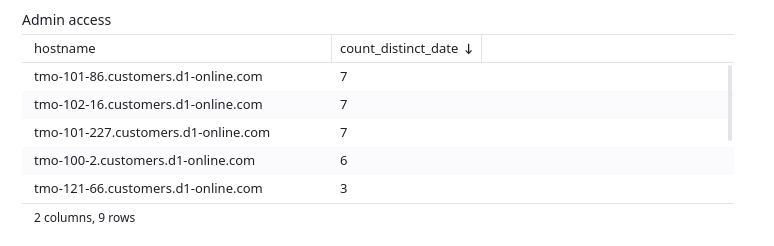
\includegraphics[width=\linewidth]{images/figure06.png}
\label{fig:adminAccess}
\end{figure}

Not surprisingly, with a few exceptions, admin access seems to come from the Deutsche Telekom network, the primary carrier in Germany. Not that this data point is of huge interest, but we can at least rest assured that we most likely were not hacked or pwned.

\subsection{Referrals}

A much more interesting data point than admin access is the referrals, this time not from the wp-search index but from the wp-visitor table itself:

\begin{figure}[H]
\centering
\caption {Referrals}
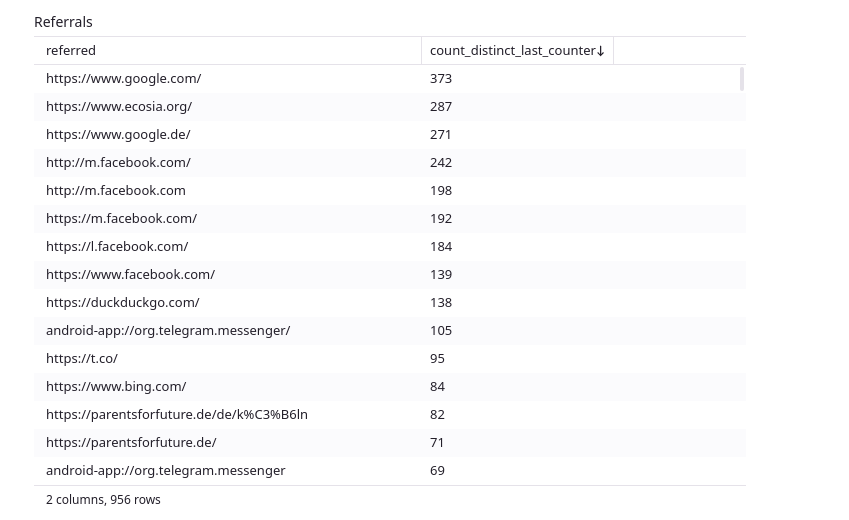
\includegraphics[width=\linewidth]{images/figure07.png}
\label{fig:referrals}
\end{figure}

We can still see Google and other major search engines in the referrals. Still, interestingly enough, the more privacy-oriented ones (\href{https://www.ecosia.org/?c=en}{Ecosia}, \href{https://duckduckgo.com/}{DuckDuckGo}) are pretty high on the list. 

In addition, we can also see several referrals from our Twitter, Facebook, and Telegram channels. It indicates a solid connection with the community and tight integration of the blog with our other social media sources, which is the blog's primary goal.

To keep the community together, to combat loneliness and climate anxiety, a strong connection through as many virtual channels as possible is vital for our outreach work.

\subsection{Platforms}

As we previously saw in the referrals, the number of people in our community using alternative search engines is relatively high. Will we see the same differences when we look at the OS and browser?

Let's start with the operating system:

\begin{figure}[H]
\centering
\caption {Operating System}
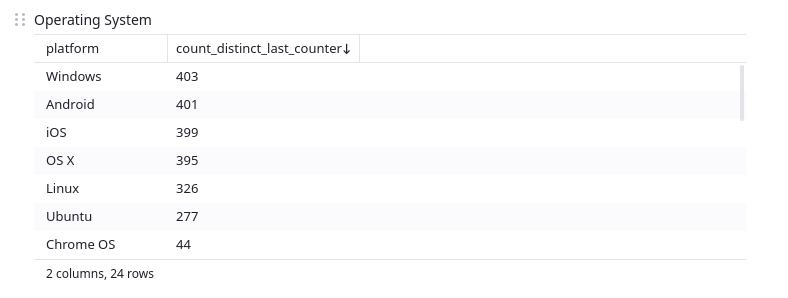
\includegraphics[width=\linewidth]{images/figure08.png}
\label{fig:operatingSystem}
\end{figure}

Access from mobile is pretty evenly split between Android and iOS, as I would expect it to be. 

However, the desktop distribution looks quite interesting: Even though Windows and Mac OS X are again pretty tight, the number of Linux users is far higher once we sum up all the distributions. It is a very different distribution from the overall distribution of desktop operating systems, where the percentage of Linux users usually is in the lower single digits.\footnote{See \textit{Frank, C. (2021)}: Web Traffic Analysis - Predicting Blog Post Performance. \cite{previousBigData}}

Now, let's look at the browser figures:

\begin{figure}[H]
\centering
\caption {Browser}
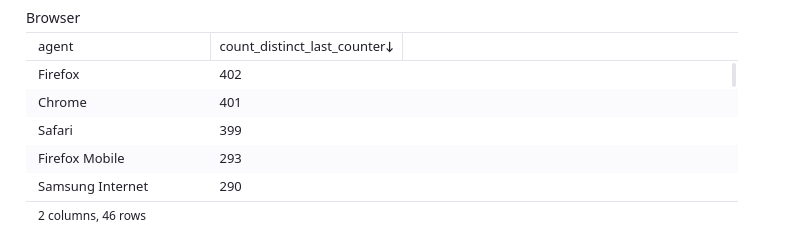
\includegraphics[width=\linewidth]{images/figure09.png}
\label{fig:browser}
\end{figure}

Again, this is a very different and exciting distribution: Firefox and Firefox Mobile together are leading the access, easily outperforming Chrome or Safari. 

This distribution is a continuation of what we saw before. Our community of climate activists does not like to rely on mainstream search engines, mainstream operating systems, or mainstream browsers.

A quick test on \href{https://webpagetest.org/}{WebPageTest} showed a significant difference in loading times and \href{https://web.dev/vitals/}{web vitals} for Chrome and Firefox. Given the high number of Firefox users on our blog, there's room for improvement here.

From the data, there are a couple of key takeaways for the future before we move on to the next chapter:

\begin{itemize}
 \item We should focus SEO more on Ecosia and DuckDuckGo, and less on Google
 \item Firefox is the most prevalent browser, on the Desktop and mobile devices, we should optimize the blog theme for it
 \item Quite surprisingly, Linux is the most favored desktop operating system; we should take that into account for all media formats, especially for images and videos
 \item Mobile access is important, even though still less than 50\%, and we should improve the interface design and speed by optimizing the theme for mobile access
\end{itemize}


%
%	Praxisbezug
%

\pagebreak
\section{Data Analysis}

\onehalfspacing

\subsection{Engagement Overview}


\subsection{Outlook}

Coming back to the original question for the paper "On which subject(s) should I post to increase my reach?" we now have a definite answer.

According to the data, posting more content on Climate Change and Covid-19 should lead to more visitors' engagement.

I'll keep that in mind for the future and change the content that I post accordingly.

Cross-posting to Facebook is an already established automated procedure, so I'll keep doing that for now. Also, I like posting in English, so I'll continue this practice as well.

I will work on the other two recommendations to improve Google search and mobile usability.



%
%	Fazit
%

\pagebreak
\section{Summary}

\onehalfspacing

From the analysis, we can see that it makes a lot of sense to focus the posts on the Kölle for Future blog on the two major crises of our time, the Climate Emergency and the COVID-19 pandemic.

Using wp-statistics for web analytics was initially an easy option, however, in case we want to continue in-depth analysis of the performance of our blog, we might consider moving to another tool or platform.

The overall result is not really a surprise, these two issues are the most talked-about issues on all media and are on everybody's mind all the time. The data showed us also some more actionable items, such as putting more focus on mobile users and is also asking us to make sure that we cater for browsers and platforms which are not mainstream.

But, most importantly, the data showed us that we can engage with the KFF community and the wider network of climate activists with the help of our blog. In times where social distancing is de rigueur, it is very important to use alternative means to reach out, means that do not require physical contact. From the past year we can conclude that digital activism works, both as a support for the community and also as way of protest. Quite surprisingly we found out that our politicians indeed pay attention to social media.

Maintaining connections during the pandemic is the most important part of combating loneliness and building up resilience, and the focus of our outreach work.

Digital Activism works!


% Literaturverzeichnis
\cleardoublepage
\raggedright
\bibliographystyle{IEEEtranS}	% ieeetran verwenden, damit auch URLs angezeigt werden
\bibliography{seminar-lit}

% \cleardoublepage
% \justify
% %
%	Ehrenwoertliche Erklaerung
%

\pagebreak

\pagenumbering{gobble} % Keine Seitenzahlen mehr
\onehalfspacing

%-----------------------------------
% Ehrenwoertliche Erklärung
%-----------------------------------
\section*{Declaration in lieu of oath}

\par\medskip

With this, I declare that I produced the submitted paper with no assistance from any other party and without the use of any unauthorized aids and, in particular, that I have marked as quotations all passages which are reproduced verbatim or near-verbatim from publications. Also, I declare that the submitted print version of this thesis is identical to its digital version. Further, I say that I have never introduced this thesis to any examination board in either its present form or in any other similar version. I herewith agree that you may publish this thesis. I herewith consent that you may upload this thesis to an external contractors' server to submit it to the contractors' plagiarism detection systems. Uploading this thesis to send it to plagiarism detection systems is not a form of publication.

\par\medskip
\par\medskip

\vspace{5cm}

\begin{table}[H]
	\begin{tabular*}{\textwidth}{c @{\extracolsep{\fill}} ccccc}
		Cologne, \the\month/\the\day/\the\year \\
		\rule[0.5ex]{12em}{0.55pt} & \rule[0.5ex]{12em}{0.55pt} \\
		(Location, Date) & (Signature)
	\end{tabular*}
\end{table}


\end{document}
